

\begin{frame}[fragile]

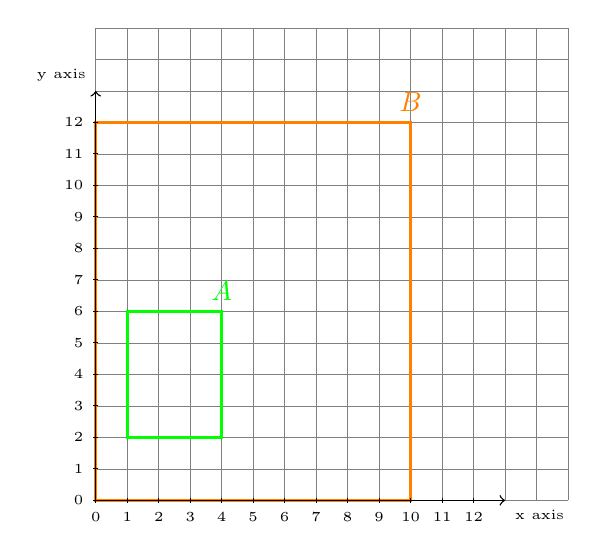
\begin{tikzpicture}
\draw[step=0.4cm,gray,very thin] (0.0,0.0) grid (6,6);
\draw[orange, very thick] (0.0,0.0) rectangle (4.0,4.8) node[anchor=south] {$B$};
\draw[green, very thick] (0.4,0.8) rectangle (1.6,2.4) node[anchor=south] {$A$};
\foreach \x in {0,1,2,3,4,5,6,7,8,9,10,11,12}
    \draw (\x * 0.4 cm,1pt) -- (\x * 0.4 cm,-1pt) node[anchor=north] {\tiny $\x$};
\foreach \y in {0,1,2,3,4,5,6,7,8,9,10,11,12}
    \draw (1pt,\y * 0.4 cm) -- (-1pt,\y * 0.4 cm) node[anchor=east] {\tiny $\y$};

\draw[->, line width=0.5pt] (0,0) -- (5.2,0) node[anchor=north west] {\tiny x axis};
\draw[->, line width=0.5pt] (0,0) -- (0,5.2) node[anchor=south east] {\tiny y axis};
\end{tikzpicture}


\end{frame}

\begin{frame}[fragile]
\frametitle{rectangle.cpp}
\begin{lstlisting}
#include "rectangle.h"

Rectangle::Rectangle(int x, int y, int width, int height)
    : x(x), y(y), width(width), height(height) {}

bool overlap1D(int a0, int b0, int a1, int b1) {
    return a0 < b1 && b0 < a1;
}

bool Rectangle::overlap(const Rectangle &other) const {
    return overlap1D(x, other.x, x + width, other.x + other.width) &&
           overlap1D(y, other.y, y + height, other.y + other.height);
}
\end{lstlisting}
\end{frame}
